\section{Analysis}
\label{sec:analysis}
The process of CERED creation is mostly an attempt to execute the first two parts of the pipeline we mention in 
\autoref{sec:relation_extraction_pipeline_proposal}. To the best of our knowledge, there is no suitable entity linking tool for Czech. There are tools for named entity recognition that we could theoretically use to our advantage, if we decided to focus on named entities only.

Therefore, we need to find a way to get to similar results as the first stages of the pipeline. We do not expect that our CERED generator will be as powerful as the respective dedicated tools would be. We do not try to create general entity recognition and linking tools -- on the contrary, we exploit all suitable extra information that chosen Wikimedia projects provide.

There are several aspects that we need to think through. We introduce them in the following list for better orientation, and then elaborate every one in more detail in dedicated subsection. 
\begin{itemize}
 \item  \textbf{Dataflow} -- we chose Wikidata and Czech Wikipedia, but we did not discuss how to connect them and what exactly should be the outcome so that we can proceed to locating mentions.
 \item  \textbf{Entity Matching} -- suppose we collected a piece of text together with a set of entities that could be mentioned in the text. The process of entity matching attempts to mark words in the text that mention an entity.
 \item  \textbf{Wikilink Mentions} -- Wikilinks are (mostly) human labeled entity mentions. Utilizing them is the closest we can get to a supervised dataset without actually supervising the dataset.
 \item \textbf{Relation Matching} -- after entities are matched in the Wikipedia texts, relationships are extracted from the Wikidata dump and we use distant supervision assumption to locate relation mentions in the texts.
\item \textbf{Relation Inventory} -- we generated CERED, but the relation inventory is overly diverse. Moreover, the dataset is extremely unbalanced -- the number of mentions per relation varies -- and we lack negative relation.
 \item  \textbf{Result Evaluation} -- every time we generate CERED during development, we need to evaluate its quality. We propose methods for this evaluation. 
\end{itemize}




\subsection{Dataflow}

We start the whole process of creating our dataset with two files. The first file is a Czech Wikipedia dump. It is a collection of articles where each article has its title, id, and text. And the other file is a Wikidata dump. 

The simplest way of processing those files would be to process them separately and thus obtaining sentences on one side and relationships (a relation type with two items) on the other. This approach comes with a clear disadvantage. We would lose any additional information about the sentences that could be potentially useful (for example article title might be helpful to determine which items are mentioned in the sentence). 

To prevent the loss of information, we could precompute additional data for each article and attach it to each sentence (article title, all Wikilinks in the article, etc.), risking a massive increase in required capacity to work with such data. On a similar note, we could process Wikidata to store item names (labels and aliases) for each relationship, worsening the situation even further.

\begin{figure}
\begin{subfigure}{1\textwidth}
\centering
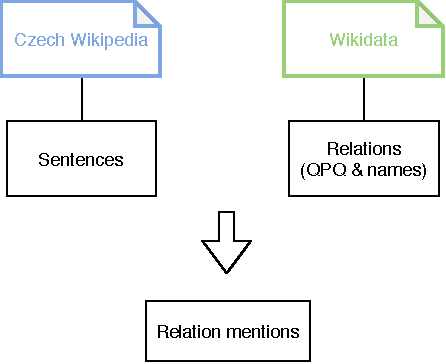
\includegraphics[scale=0.8]{./img/Diplomka diagramy-uninformed} 
\caption{Uninformed approach of locating mention relations in text}

\label{obr:uninformed}
\end{subfigure}

\par\medskip
\qquad
\begin{subfigure}{1\textwidth}
\centering
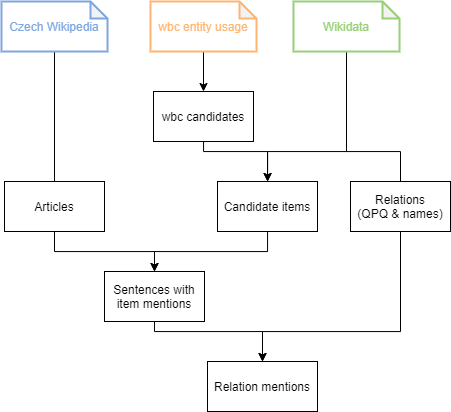
\includegraphics[scale=0.8]{./img/Diplomka diagramy-informed} 
\caption{Informed approach of locating mention relations in text}

\label{obr:informed}
\end{subfigure}

\label{obr:informedvsuninformed}
\end{figure}


\todo{Popisky u obrázku informed and uninformed}
We decided to update the dataflow to address those issues. We preprocess the Wikidata dump to contain only the data we use. We refer to this processed version of Wikidata as \defineterm{custom Wikidata}. An item is kept only if it has a Czech name and we significantly reduce its statements: we keep the title of its Czech Wikipedia article and create a list of (QID,PID,QID) triples, \defineterm{QPQ}, representing statements that contain information about relations between this item and other items. This way, we have all the necessary information -- article title to be able to connect an article to an item, names for each item to be able to find mentions of items, and finally QPQ triples to connect relations and sentences. Moreover, custom Wikidata size is closer to traditional RAM size. Therefore we could for example load item names into memory, which comes in handy during the implementation.

One approach to finding item mentions in text could be called uninformed (Figure \ref{obr:uninformed}). We could assume that any item can be mentioned in any sentence. This approach has two issues: the computation would likely take quite some time, but mainly we expect a huge amount of ambiguous mentions. An example of this ambiguity, which we see as problematic, might be children named after their parents. In this case, not only that the entities might get confused, but also if we then assign the relation, we might easily confuse a sentence mentioning a spouse relation for a parent relation, which, unfortunately, is extremely challenging to solve. 

On the other side, we can use the extra information that Wikimedia projects provide and opt for a more informed approach. A diagram of this approach is captured in \autoref{obr:informed}. The topic of most Czech Wikipedia articles is a Wikidata item, therefore this item is nearly certainly mentioned in the article. Some Wikidata statements were based on relevant articles and thus it seems plausible to expect that items related to the main item of an article are mentioned in it. We, therefore, decided to look only for a tiny subset of all Wikidata items in each article, the so called \defineterm{candidate items}, which consist of the article item and all times connected to it by a statement.


Czech Wikipedia maintains a \verb|wbc_entity_usage| table, which contains information about which article uses which item. If we use this table, we are able to obtain a list of items, that should be mentioned in an article, let us call this list a \defineterm{wbc candidates}. A wbc candidate is at the same time a candidate item.

We might consider adding even a second level of relatives (items related to items that are related to the main item), but the branching factor might be relatively high and cause unwanted ambiguity. Consider an instance item like a specific country, all countries would be second level relatives and thus candidate items. Since countries tend to be of a certain type (kingdom, republic, state etc.), there might be simply the type or some other more general name amongst their names (\wikiitem{United States of America}{Q30} are also known as America or United States) and more countries might share this name.

So far we mostly discussed the advantages of the proposed informed approach, mainly a hope for higher precision, specifically higher precision for item mentions. We should elaborate on some disadvantages as well. We are not trying perform fully do entity linking. In the end we will only use item mentions, if the following condition holds: there are two entity mentions in one sentence and there exists a QPQ that connects them. It is questionable whether we need an informed approach to increase relation mention precision. The improbability that this condition is fulfilled for false-positive item mentions might in fact be sufficient.

One more way to locate item mentions is through \defineterm{Wikilinks}. A Wikilink links a page to another page within the same-language Wikipedia. First additional information this brings is simply the item mention (if the linked page or article has its main item). We can also consider the textual part of the link to be another name for the linked item. The quality and suitability of this name are to be examined and if we find these names useful, they can be added to the item names we use.


\subsection{Entity Matching}

We have text on one side, gathered candidate items on the other side and our goal is to find occurrences of these items in the text. We call this process \defineterm{entity matching} and each found occurrence is an \defineterm{entity mention}.

No matter how the matching is done, it seems always beneficial to start the process with some text preprocessing. Quite a lot of changes need to happen even if some seem like little details. We separate this preprocessing into a wiki specific part, lexical analysis, and the last part is devoted to lexical analysis on standalone noun phrases.

When we eventually proceed to entity matching, there is a wide spectrum of complexity we might aim for. Bearing in mind that we are no trying to create a strong sophisticated tool for entity recognition and linking., we describe some of those levels of complexity and choose the right method for our use case.



 

\subsubsection{Wikipedia parsing}
\label{sec:wikipedia_parsing_analysis}
Wikipedia parsing starts with an article in Wikitext and produces human-readable plain text -- a \defineterm{clean text}. Note that we should keep track of positions of Wikilinks from the Wikitext in the clean text.

Wikipedia is written in Wikitext (Wiki markup, Wikicode). This markup provides all usual functionalities such as determining the layout or fonts, and enables commonly-used concepts like lists, links, media file insertion, or tables, and some more wiki specific concepts like infoboxes.

We plan on using one or even a combination of existing Wikitext parsers, since each of them provides different functions.\footnote{\url{https://www.mediawiki.org/wiki/Alternative\_parsers}} Therefore the parsing itself is not too troublesome. 

One problem that needs to be addressed is what should we consider a valid text. For example, it is not clear how to work with tables. From one point of view, if we convert a table into an unstructured text, it will not be a regular text in terms of sentence structure. From a different point of view, an unstructured text obtained by converting a table still contains information that human readers will likely decode. Moreover, tables and other structured data tend to contain a lot of information. This will likely cause problems, because we want to concentrate on sentence-like data. For example, pairs of persons and countries might be matched from sport results tables. This kind of data might significantly damage the quality of CERED.

The elimination of all Wikipedia content that is too structured or generally not enough sentence-like, but at the same keeping as much as possible, is addressed later in \autoref{sec:wikiperia_parsing_implementation}. That way we can see the consequences of the eliminated and kept content.


\subsubsection{Lexical Analysis}
Keeping text (such as an article) in long sequences of characters is not the best format for our purpose. Instead we need to parse those sequences into smaller units, such as words and sentences. A tool that addresses such tasks is usually called a \defineterm{tokenizer} and a \defineterm{token} is a term generalizing the term word. Often words in text are the same as tokens, but \vuvozovkach{aren't} in English and \vuvozovkach{mohu-li} in Czech are likely considered one word but multiple tokens. On the contrary, \vuvozovkach{M*A*S*H} or \vuvozovkach{email@email.com} might not be considered a word, but should be considered exactly one token each. Naive tokenizer might just simply split on non-alphanumeric characters,but for better performance, a more sophisticated tool is needed. 

Since we work with Czech, which is a language with rich morphology, we might want to know non-inflexed form of a token, moreover we might want to assign some unique idintifier to such form in case it has some homographs (words that are spelled the same way). Such am identifier is called a \defineterm{lemma} and a collection of tokens that share the same lemma is called a \defineterm{lexeme}. 
We outsource handling text to a Czech tokenizer and tagger called MorphoDiTa \citep{Morphodita}, that achieves state-of-the-art results for the Czech language. Using such a tool, we can convert clean text into sentences made up of tokens and we even obtain the lemma and lexeme of each token.

\subsubsection{Lexical Analysis on Names}
Tokenizers (and lemmatizers) are usually trained to perform well on sentences and might be inaccurate on noun phrases when they stand alone, as entity names do. If we were determined to tokenize them, a simple trick like constructing a sentence with the name in it and tokenizing this sentence can partially solve this problem. Such a sentence that would be grammatically correct and not semantically terrible could be something like  \vuvozovkach{This is /name/}, but realistically, this sentence was quite likely not at all common in the training process of MorphoDiTa. Some foreign words can be erroneous as well and keeping their original form might be the only easy way around it.

\subsubsection{Matching methods}
Entity matching can be performed with various degrees of sophistication. We provide a short overview of four such degrees. The degrees 1 and 2 do not require any knowledge of the language they work with, while 3 and 4 are language dependent. For simplicity, we assume that we are only looking for mentions in one sentence at a time, unless written otherwise. We also include an example of such matchings to demonstrate how successful we expect them to be.



\subsubsub{1 String equality} This method is the easiest method of entity matching. It is based on a simple substring check, which is later extended with additional functionality. In more detail, for each entity, we have multiple name variants and for each of those names, we check whether the name is a subsequence of the sentence tokens.



We also need to consider the letter cases. Named entities should have fixed letter cases and no additional processing is needed in most cases. In other cases, an established name for a named entity might be written with the lowercased first letter -- \wikiitem{Weasley family}{Q716534} has Czech names \vuvozovkach{Weasleyovi} (the Weasleys) and also \vuvozovkach{rodina Weasleyových} (Weasley family). If we consider entities that are commonly written with lower case, the sentence now needs to be preprocessed so that for example the first letter is not capital. Moreover, there is no guarantee that common names will be lowercased in Wikidata. To conclude, nearly nothing can be assumed about the case of letters, and therefore one of the following solutions needs to be implemented: we can convert everything to one chosen letter case or we need to perform some more sophisticated attempts at predicting, which words can have more versions in terms of letter cases.

Another problem that we encounter is how to properly handle spaces. We list some troublesome examples and accept the fact that not everything can be done perfectly. J. K. Rowling has J.K.Rownling as one of Wikidata names, confirming that both versions might appear in written text, but not all entities with similar name type have all space-variants listed in names. We, therefore, assume that spacing around the \vuvozovkach{-} character might vary.

It is also not clear if word order in entity names is fixed (or at least almost always fixed). Even a simple reversion in name will affect the performance of this method (J. K. Rowling and Rowling, J. K.).

\begin{figure}
\centering
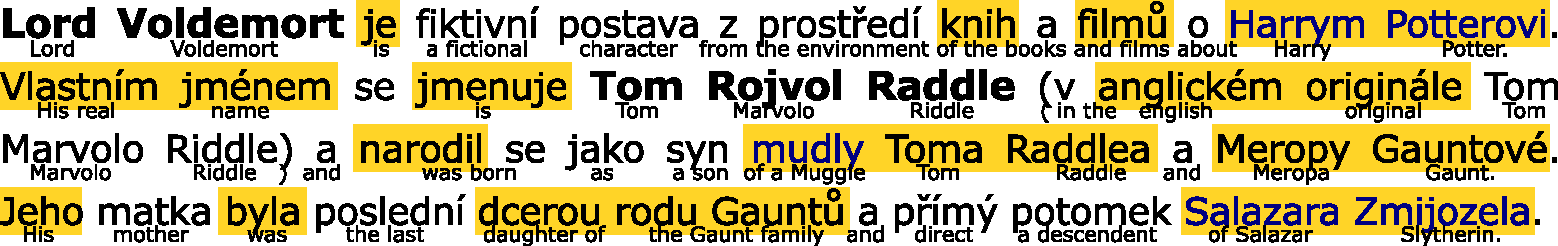
\includegraphics[width = 0.9\textwidth]{./img/Voldemort_infinitivy_preklad}

\caption{First paragraph from Czech Wikipedia page about \wikiitem{Lord Voldemort}{Q176132}, also known as \vuvozovkach{Tom Rojvol Raddle} (Tom Marvolo Riddle), \vuvozovkach{Voldemort} and \vuvozovkach{Pán zla}. Highlighted words are not in their base forms. }
\label{obr:Voldemort_preklad}

\end{figure}

The greatest weakness of this method is its inability to recognize entities if their name is inflected. To emphasize how many words are not equal to their lemma in Czech text, we colored them in a sample text presented in \autoref{obr:Voldemort_preklad}. We elaborated on Czech language in \autoref{sec:Czech}, but just for simplicity -- in English the verb \vuvozovkach{to be} has many different forms (am, are, were, was, would and so on), and in Czech all nouns and verbs behave like this, quite often with many more forms. 

To illustrate the effect of the described method, \autoref{obr:Voldemort_string_equality} displays the resulting entity mentions on a sample text.


\begin{figure}[h]

\centering
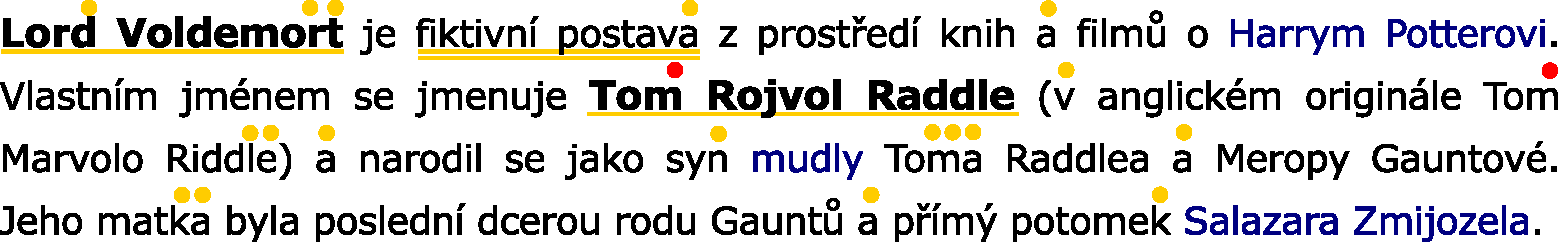
\includegraphics[width = 0.9\textwidth]{./img/Voldemort_string_equality}

\caption{Results of entity matching using string equality on the first paragraph from Czech Wikipedia page about  \wikiitem{Lord Voldemort}{Q176132}, also known as \vuvozovkach{Tom Rojvol Raddle} (Tom Marvolo Riddle), \vuvozovkach{Voldemort} and \vuvozovkach{Pán zla}. Dots represent found mentions on a single word, red stands for five found mentions, lines represent found mentions of noun phrases (five Wikidata entities match \vuvozovkach{Tom}, and one Wikidata entity matches the whole \vuvozovkach{Tom Rojvol Raddle}).}
\label{obr:Voldemort_string_equality}

\end{figure}

\subsubsub{2 String similarity (approximate string matching)} String similarity is still based on simple string manipulation, no vocabulary or other language knowledge is necessary. The goal is to find entity mention, even if its name is a little altered in the sentence. This alternation can include all of the issues listed for the previous method -- cases of letters, spacing, word order, and word forms, but even better, it might help in cases that we did not anticipate.

There are many metrics describing string similarity. Some can cope better with word order issues, some with word forms, some with spacing. We do not test all of them for our usecase, but still find it useful to mention them, since in other than the Czech language, some might work well.

First category of string similarity metric is based on \textbf{edit distance}. Levenshtein distance is the minimum number of edits (additions, deletions, and substitutions of a character) to get from one string to the other. As a metric the ratio of Levenshtein distance and of the sum of the lengths of the strings can be used. This metric, unsurprisingly, handles well the mentions that are close in the amount of edits needed, so mentions with different inflection, spacing, or letter casing will likely be considered a match.

Damerau–Levenshtein distance is very similar to the previous, but a transposition of two adjacent characters is also considered an edit. We might argue that some Czech words tend to transpose the last characters in different word forms and thus this metric could work better for those forms, but there might be a higher risk of false positives.


Another category is \textbf{based on tokens}. The tokenization converts both the sentence string and the name string into a sequence of tokens. If we consider those sequences to be sets ($S, N$ respectively), metrics that work with sets can be utilized. For example, Jaccard index (intersection over union) is computed as $|S \cap N| / |S \cup N|$. Any other set similarity measure can be used. 

Set based metrics ignore the order of tokens and therefore could solve issues with mentions in which the word order is not the same as in the name. On the other side, an increase in false positives is to be expected, and some additional post-processing is needed to determine which token in the sentence should be considered a mention, if the token was used in the sentence multiple times. 


%\subsubsub{3 Sequence based} Just to be a bit more comprehensive, we include another type of metrics - sequence based, even though we doubt it is the best approach for entity matching. They ignore words as wholes and we do not see any advantage of those metrics for our use case. 

%Ratcliff-Obershelp similarity finds the longest common substring that is longer than some limit and recursively does so for the non-common parts of strings. The result is based on the ratio of (double the) length of common parts and overall length. 

%Bigram (or n-gram) intersection over union which converts both strings into a set of n-grams (n adjecant characters) and performs intersection over union. This time reducing a sentence into a substring is not that straight forward and would require additional attention.



\subsubsub{3 Morphological analysis}
Moving on from methods that are mostly unaware of the language they work with, we will finally use the \textbf{morphological analysis} we mentioned earlier.

With lemmas of both the sentence and the name, we can use any metric from the previous subsection on string similarity (joining the lemmas using a space if the metric expects only two input strings).



\begin{figure}[h]\centering
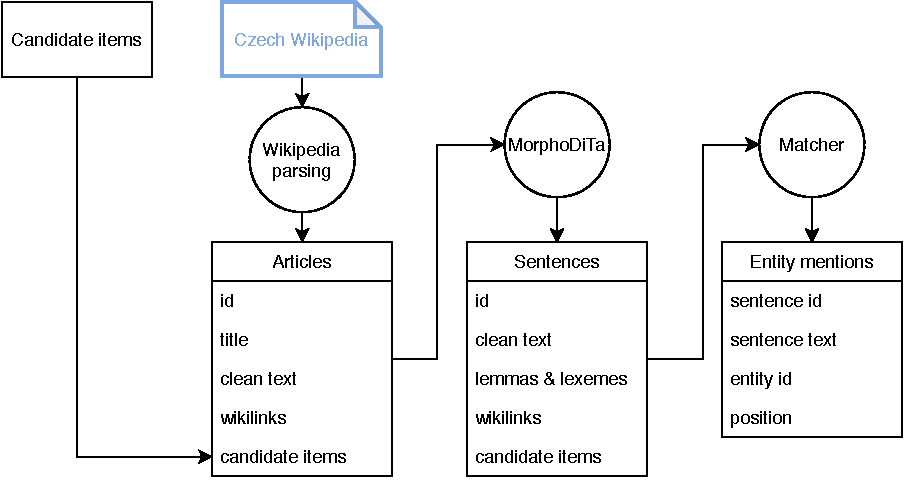
\includegraphics[width=0.9\textwidth]{./img/Diplomka diagramy-Detailed_text}
\caption{Matching with morphological analysis}
\label{obr:DiagramTextDetail}
\end{figure}

If we decide to keep the entity names in their original form (tokenization on them can be error prone, as we already explained), we can try to use the correct form of the tokens in the sentence. For each word in the sentence, we use its lexeme to determine if (part of) a entity name matches the word.

Detailed diagram of matching entities using morphological analysis is shown in \autoref{obr:DiagramTextDetail} and the obtained results on the sample text are captured in \autoref{obr:Voldemort_morpholo}.


\subsubsub{4 Advanced concepts} Proper entity matching (either in named entity recognition or entity linking) might be expected to recognize entity mention even if the entity is not mentioned explicitly by its name. Pronouns should be assigned an entity they represent (if they do) and other nouns as well. In languages like Czech, where the subject of a sentence is often omitted, the entity mention is even less obvious, but still present. Since the topic of this thesis is not entity matching, we will not debate techniques to achieve this level of matching neither will we implement them.


\begin{figure}
\centering
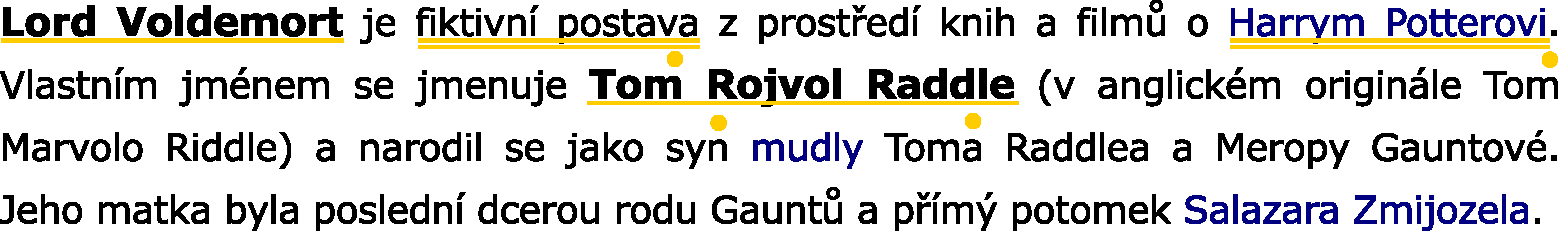
\includegraphics[width = 0.9\textwidth]{./img/Voldemort_lexical}

\caption{Results of entity matching using morphological analysis and informed approach on the first paragraph from Czech Wikipedia page about  \wikiitem{Lord Voldemort}{Q176132}, also known as \vuvozovkach{Tom Rojvol Raddle} (Tom Marvolo Riddle), \vuvozovkach{Voldemort} and \vuvozovkach{Pán zla}. Dots represent found mentions on a single word, lines represent found mentions of noun phrases (one candidate entity matches \vuvozovkach{Tom}, and one one candidate entity matches the whole \vuvozovkach{Tom Rojvol Raddle}). }
\label{obr:Voldemort_morpholo}
\end{figure}

\todo{obrázky jsou špatně, zase}


\subsubsection{Conclusion}
After looking at the results, we decided to use a simple metric based on morphological analysis -- a detailed description of the matching method CERED was generated with is described in \autoref{sec:entity_matching_implementace}. We still find it useful to keep this summarization of different string metrics as part of this thesis.


\subsection{Wikilink Mentions}

As we already mentioned, from our point of view, Wikilinks are entity mentions created by Wikipedia editors. The text part of the link can in theory be anything, providing us with some more advanced examples of entity linking that our matching methods cannot perform.

Since this data is not fully supervised and the word supervised is overused (semi-supervised, distant-supervised, etc.) we decided to call it \defineterm{silver}, because they are not of the optimal quality that is usually called gold, but they are the best we can get.


\subsection{Relation Matching}
If a sentence contains two entity mentions that are related, chances are that the sentence in fact does express their relationship and thus is a relation mention. This concept is called \defineterm{distant supervision assumption} and can be also formulated in the following way: If two entities participate in a relation, all sentences that  mention these two entities express that relation. This assumption is commonly used, even though it is clearly not correct, because it is easy to use. 

To evaluate, how often this assumption is violated, is labour-intensive, but luckily is has already been performed. In \cite{nytdistant}, the distant supervision assumption is compared to the \defineterm{express-at-least-once assumption}, which states that if two entities participate in a relation, at least one sentence that mentions these two entities might express that relation. 

The authors sampled 600 relation mentions from two corpora, both created by distant supervision on Freebase (knowledge base commonly used before Wikidata took over) and two text corpora - Wikipedia articles and the New York Times corpus. These 600 samples represented three different relation types (\relationtype{nationality}, \relationtype{place of birth}, and \relationtype{contains}) and were sampled so that there were 100 samples of each type in each corpus. We include their results in \autoref{table:nytvswikiDS}. They concluded that the distant supervision assumption holds more often in Wikipedia because Wikipedia is a very specific type of text corpora, where articles are centered around entities. We believe that the reasoning can be extended with the fact, that Freebase contained information from Wikipedia infoboxes, and those infoboxes were created based on the textual information. 

\begin{table}[h]
\centering
\begin{tabular}{ l c c }
\hline
 & NYT & Wikipedia\\
\hline
\hline
\relationtype{nationality} & 38\% & 20\% \\
\relationtype{place of birth}  & 35\% & 20\% \\
\relationtype{contains}  & 20\% & 10\%\\
\hline

\end{tabular}
\caption{Percentage of times a related pair of entities is mentioned in the same sentence, but where the sentence does not express the corresponding relation. Taken from \cite{nytdistant}.}
\label{table:nytvswikiDS}
\end{table}


For the authors the results signalized that a more sophisticated tool is needed, instead of relying on the distant supervision assumption. We acknowledge that such a tool is needed, but at the same time, we believe that in our case, where we create CERED based on Wikipedia and Wikidata, the precision they estimated is sufficient. We also assume, that Wikidata project is more suitable for this task than was Freebase.

We want to mention, that we build CERED to easily fit into the modern deep learning models and to be as simple as possible. Therefore, the main unit of text we use is a sentence, which is intuitive, but it has one downfall -- the resulting relationship extractor cannot detect relations expressed over sentence boundaries.


\subsection{Relation Inventory}
In \autoref{chap:datasets} three examples of relationship extraction datasets were introduced. The creators of those datasets claim, that in the creation process, they first decided on the relation inventory (relation types).  Creating the relation inventory seems to be the straightforward and rational approach, and we wanted to create such inventory before actually implementing the CERED generator. However, we stumbled upon the following issues.

\subsubsection{Huge Wikidata Relation Inventory}Wikidata relation inventory (properties in Wikidata terminology) is an order of magnitude larger compared to the traditional relationship extraction datasets and handpicking our inventory is overwhelming. We even considered reducing the size of this inventory by creating our own relations that would combine Wikidata relations (parent would be a combination of mother and father relations). 

Given the excessive number of Wikidata relation types, we decided to considerably reduce them. However, to not omit the best-represented relations, we constructed the relation inventory only after the creation of CERED.


\subsubsection{Absence of a Negative Relation}Knowledge bases, in general, do not contain negative relations (relations that could be easily mapped to the \relationtype{no relation} or \relationtype{other relation}), but for relationship extraction, negative mentions are essential. If we generate mentions using all properties, we can later decide which relationships will be in the inventory and the rest of them relabel to \relationtype{other relation}. If we were to assign all tuples of entity mentions that share a sentence and are not related as \relationtype{no relation}, we could increase the noise in CERED, because not all relationships are in Wikidata and therefore some of the \relationtype{no relation} mentions could in fact be positive mentions. The ratio of negative and positive mentions in the two bigger datasets we introduced in \autoref{chap:datasets} were approximately 80\%.

While curating the inventory, we should keep in mind, that we are not just choosing the relations, but also their representations, and we need to attempt to fulfil the three following requirements to the best of our abilities:
\begin{itemize}
\item Each relation needs to be represented enough.
\item The more balanced relation representation the better.
\item There should be enough negative mentions and their negativity should be assured.

\end{itemize}

\subsection{Result Evaluation}
\label{sec:analyzaevaluace}
The most challenging aspect of working with Czech Wikipedia and Wikidata is their size and diversity. To the best of our knowledge there is no strictly followed guideline, when it comes to editing either the articles or item information. Just converting Wikipedia dump to clean text is challenging, due to user defined templates and other constructs we might be unaware of. On the other side, names in Wikidata can be too general (like someone's first name) and create false entity mentions. 

Any change we make in the generator affects the generated dataset and analysing the consequences is difficult. We used several methods to measure the quality of the implemented generator.

The simplest characteristic of the dataset is its size. Even though we want to maximize the size of dataset, we want to keep the precision high (eliminate false positives).

We can find false positives by finding anomalies in the dataset. We can look at different graphs characterizing the dataset, identify unexpected peeks and investigate the mentions causing them. An example of such graph is the distribution (histogram) of the number of words in a sentence and article representation is shown in \autoref{obr:ukazka_histogramu}. Other useful characteristics include the length of a sentence in characters, relation distribution, article distribution, the number of sentence within its article, and so on.

Such graphs are better at capturing false positives than false negatives. To evaluate false negatives, it is necessary to compare the articles with the corresponding mentions in the dataset. To that account, we created a tool, which can visualize the whole article and both the entity and relation mentions.

\begin{figure}
\begin{subfigure}{1\textwidth}
\centering
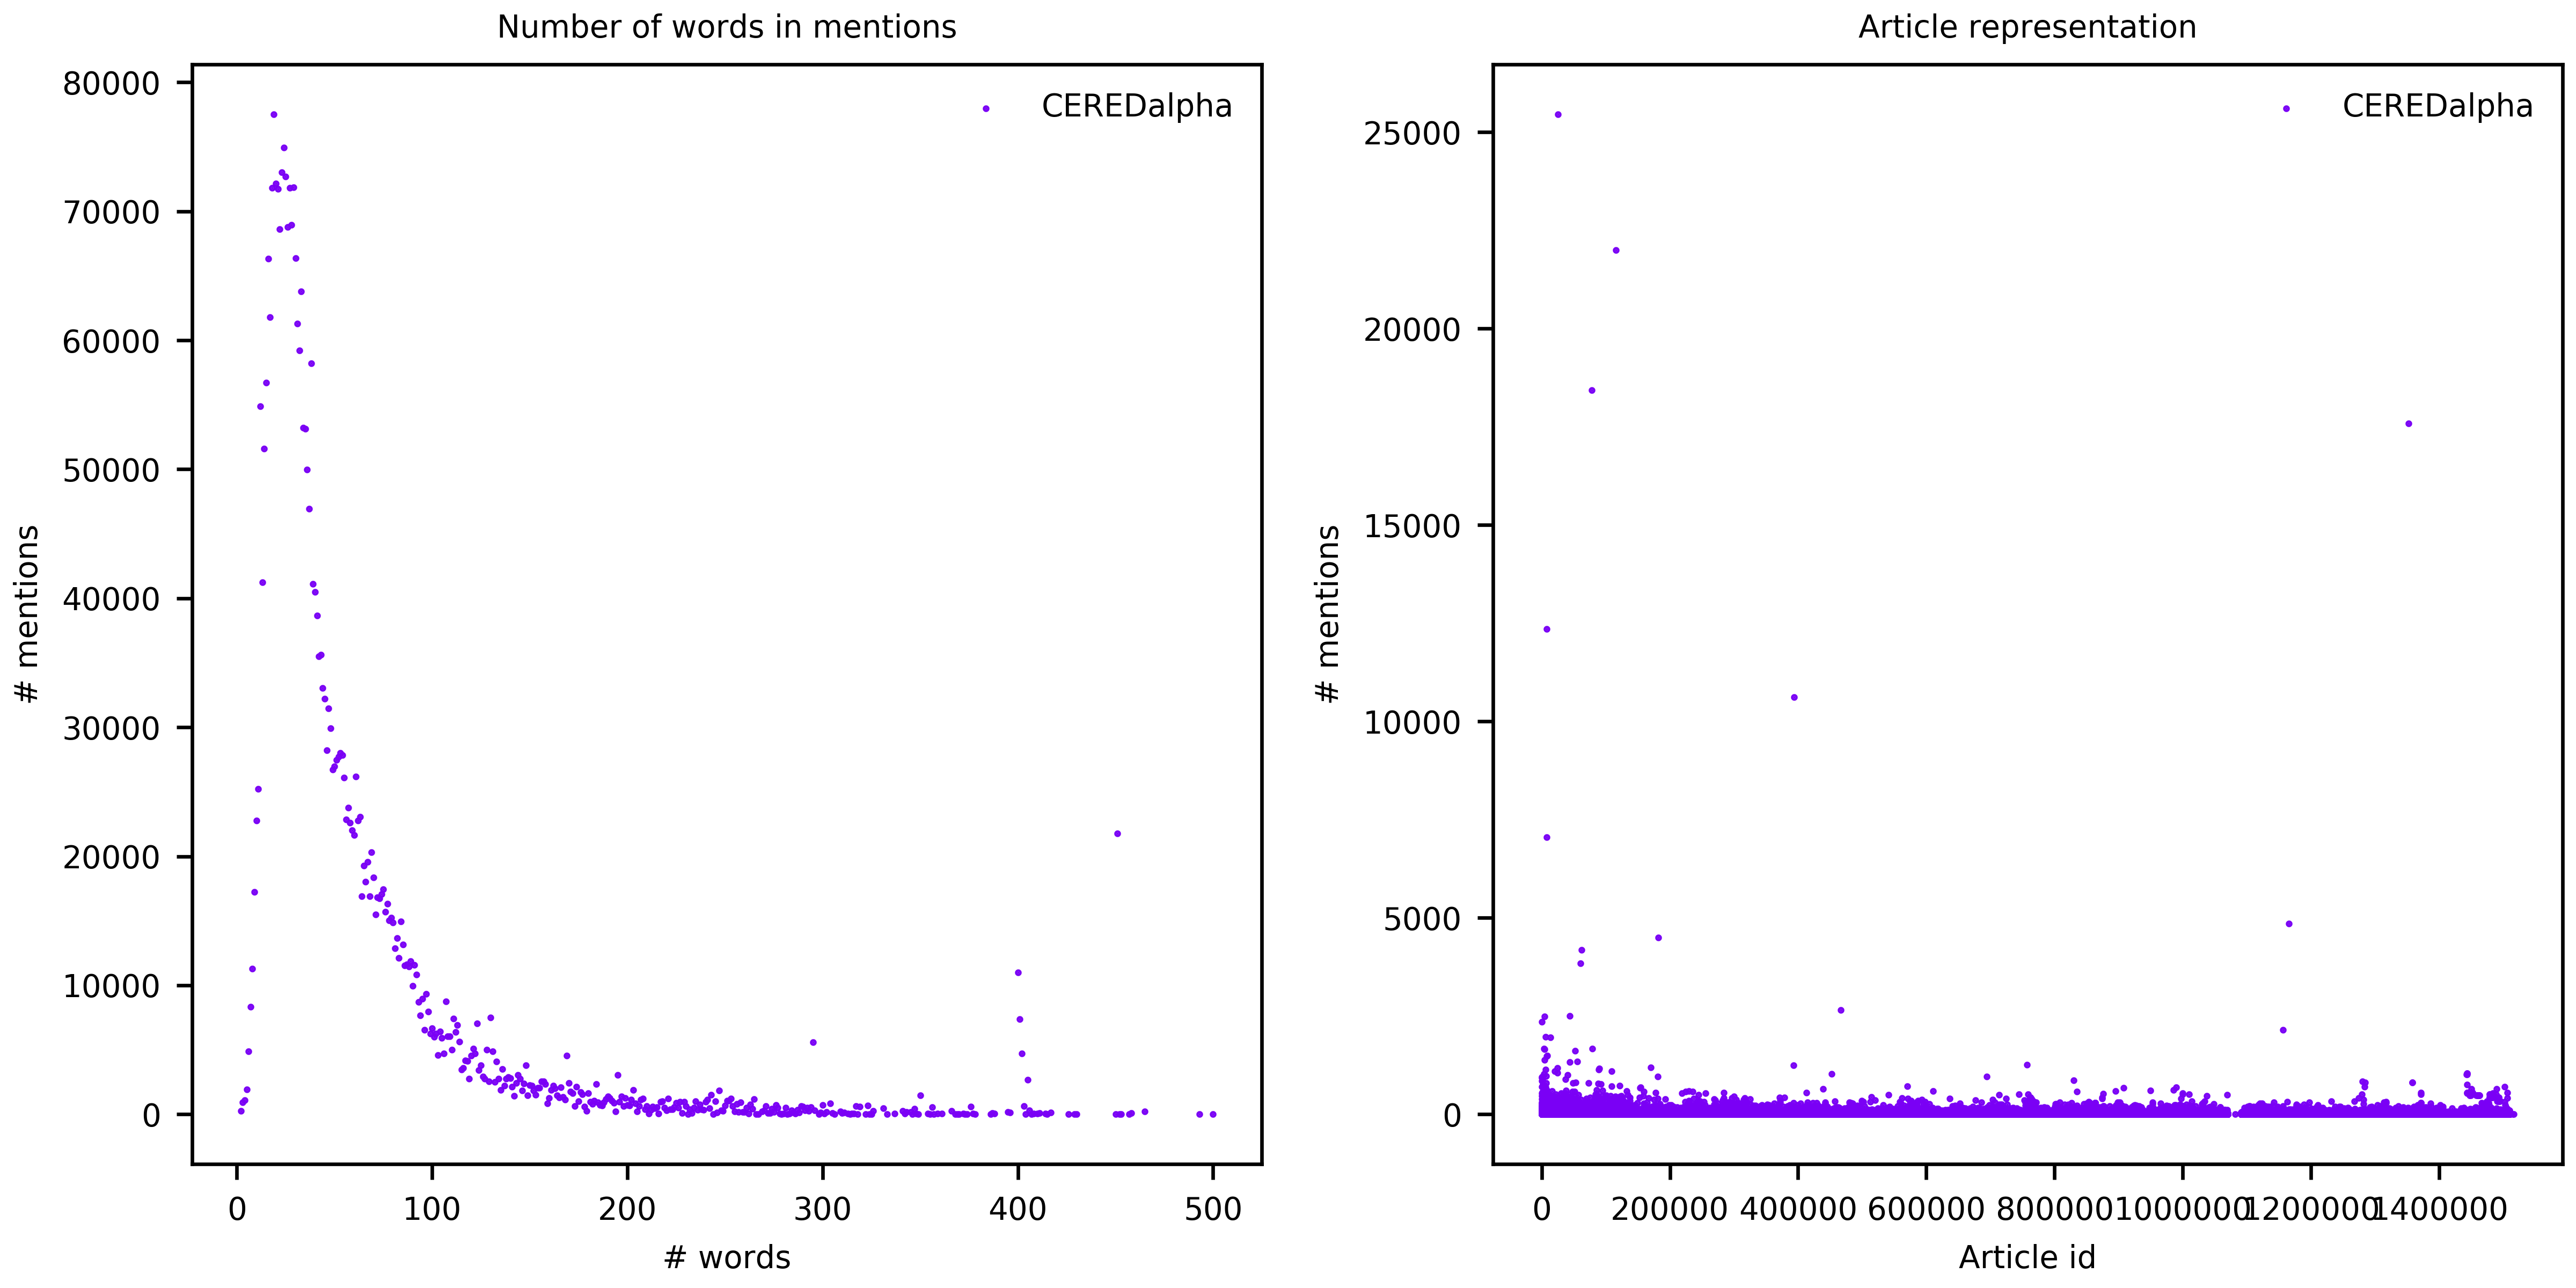
\includegraphics[width = 1\textwidth]{./img/Histograms_2020-07-19_21-00-53_CEREDalpha.png}
\caption{CEREDalpha -- alpha version of the dataset before we removed Wikitext templates}
\end{subfigure}
\par\medskip
\begin{subfigure}{1\textwidth}
\centering
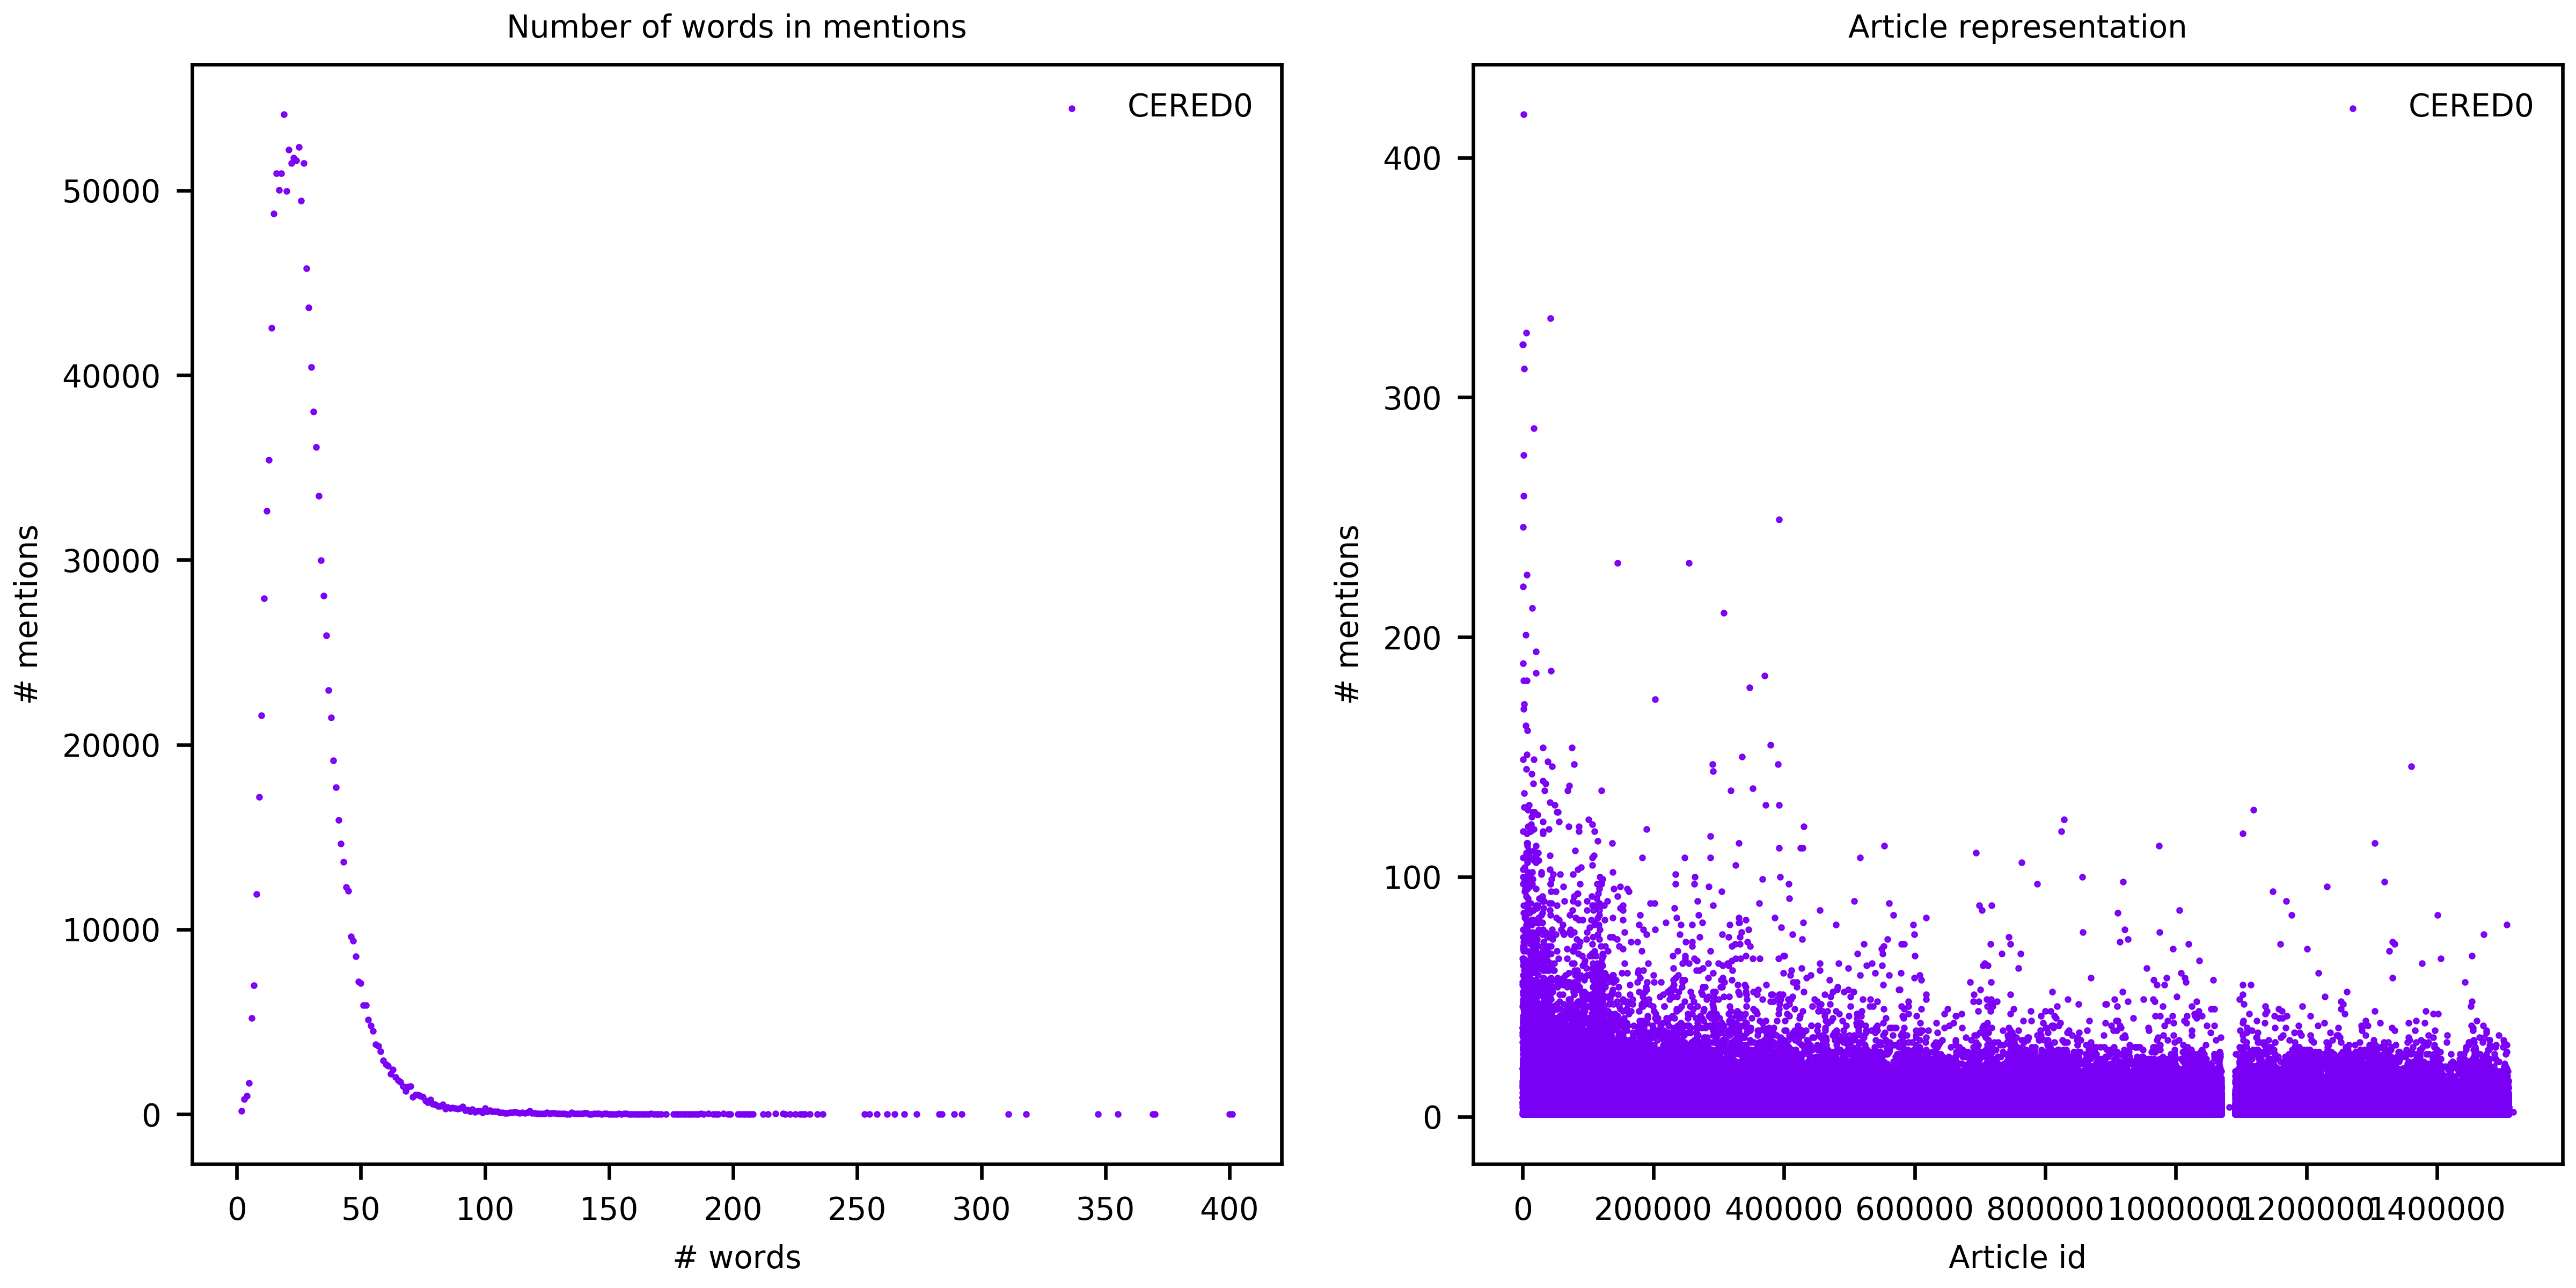
\includegraphics[width = 1\textwidth]{./img/Histograms_2020-07-19_21-00-53_CERED0.png}
\caption{CERED0 -- the final version of the generated dataset}
\end{subfigure}
\caption{Comparison of the histogram of the number of words (left column) and article id (right column) in two different versions of the dataset. In the left column, we can see that the curve is smoother and also less skewed to the right in CERED0. In the right column, we can see that in CEREDalpha several articles contributed over 5000 mentions, in contrast with the maximum contribution of approximately 400 mentions in CERED0. Considering that CEREDalpha is approximately two times bigger than CERED0, such smoothing of the distribution is significant.}
\label{obr:ukazka_histogramu}
\end{figure}

Originally, we wanted to manually label entity mentions and relation mentions on some articles and use them to automatically evaluate the generator. However, we encountered many challenges when we tried to create such manual dataset, the main three are:
\begin{itemize}
\item the selected articles should represent Wikipedia (for example, articles about people are very different from articles about sport matches);
\item to label entity relations, we need gold entity linking, which we must create ourself -- that is challenging both because of the vast number of Wikidata items and because it is difficult to draw the line of what we expect to match (in the \autoref{obr:Voldemort_preklad} example, the \vuvozovkach{prostředí knih a filmů o Harrym Potterovi} clearly mentions the \wikiitem{Harry Potter universe}{Q5410773} and Voldemort is a ommited subject of the second sentence);
\item it is time consuming to look for relations in Wikidata, due to the large number of relations.


\end{itemize}




